%% Load document class fithesis2
%% {10pt, 11pt, 12pt}
%% {draft, final}
%% {oneside, twoside}
%% {onecolumn, twocolumn}
\documentclass[12pt,final,oneside]{fithesis2}

%% Basic packages
\usepackage[english]{babel}
\usepackage{cmap}
\usepackage[T1]{fontenc}
\usepackage{lmodern}
\usepackage[utf8]{inputenc}
\usepackage{graphicx}

%% Additional packages for colors, advanced
%% formatting options, etc.
%\usepackage{color}
%\usepackage{microtype}
\usepackage{url}
%\usepackage{cslatexquotes}
%\usepackage{fancyvrb}
%\usepackage[small,bf]{caption}
\usepackage[plainpages=false,pdfpagelabels,unicode]{hyperref}
%\usepackage[all]{hypcap}

\usepackage{amsmath}
\usepackage{amsfonts}
\usepackage{amsthm}
\usepackage{galois}

\theoremstyle{definition}
\newtheorem{definition}{Definition}
\newtheorem{example}{Example}

\usepackage{listings}

\lstset{
    basicstyle=\small\ttfamily,
    captionpos=b
}

\usepackage{tikz}
\tikzstyle{block} = [rectangle, draw, text centered, rounded corners]

\newcommand\emptypage{\newpage\null\thispagestyle{empty}\newpage}

\setcounter{tocdepth}{3}

%% Fix long URLs in DVIs
%\usepackage{ifpdf}

%\ifpdf
%\else
%  \usepackage{breakurl}
%\fi

%% Packages used to generate various lists
%\usepackage{makeidx}
%\makeindex

%\usepackage[xindy]{glossaries}
%\makeglossary

%% Use STAR and CIRCLE signs for nested
%% itemized lists
%\renewcommand{\labelitemii}{$\star$}
%\renewcommand{\labelitemiii}{$\circ$}

%% Title page information
\thesistitle{String abstract domains}
\thesissubtitle{Master's thesis}
\thesisstudent{Bc. Matej Šuta}
\thesiswoman{false} %% Important when using Slovak or Czech lang
\thesisfaculty{fi}  %% {fi, eco, law, sci, fsps, phil, ped, med, fss}
\thesislang{en}     %% {en, sk, cs}
\thesisyear{Spring 2013}
\thesisadvisor{Mgr. Karel Klíč}

%% Beginning of the document
\begin{document}

%% Front page with a logo and basic thesis information
\FrontMatter
\ThesisTitlePage

\emptypage

%% Thesis declaration (required)
\begin{ThesisDeclaration}
  \DeclarationText
  \AdvisorName
\end{ThesisDeclaration}

%% Thanks (optional)
\begin{ThesisThanks}
My thanks go to my thesis supervisor Karel Klíč for his guidance. Secondly,
I would like to thank my colleagues in his study group, Jan Dupal and
Tomáš Brukner, for thought-provoking discussions. Last but not least, I want
to thank my family and friends who supported me during the writing of this
thesis. I would not have made it without them.
\end{ThesisThanks}

%% Abstract (required)
\begin{ThesisAbstract}
This thesis is about ...
\end{ThesisAbstract}

%% Keywords (required)
\begin{ThesisKeyWords}
static analysis, abstract interpretation, abstract domain, string,
prefix, suffix, trie
\end{ThesisKeyWords}

%% Beginning of the thesis itself
\MainMatter

%% TOC (required)
\tableofcontents


\chapter{Introduction}

Computers have followed Moore's~law~\cite{Moore65-1} for more than
four decades now. Hardware gets more powerful and complex. Consequently,
software becomes more complex too. It has to be designed
with maintainability and reliability in mind. Therefore several software
verification methods have been created. Abstract interpretation is one
of them.

There are many aspects of a computer program that may be analyzed by
abstract interpretation. The focus of this thesis is how program manipulates
strings. A string is very flexible data structure that allows programmer
to represent practically anything. In fact, most of the programs written
today have to deal with strings in some form. Thus, it is important to know
how programs treat strings.

This thesis describes string abstract domains in the context of abstract
interpretation which is a framework described by Cousot~\cite{CousotCousot77-1}
\cite{Cousot00-1} \cite{CousotCousot92-4} \cite{CousotCousot99-1} and other
authors. The goal of the thesis is to design, implement and integrate several
abstract domains for strings into \texttt{canal} abstract interpreter.
\texttt{canal} is a tool designed to analyze behavior of application programs
written in \texttt{C}.

The text has the following outline: chapter \ref{chap:staticanalysis} shows
techniques currently used for improving the quality of software and static
analysis in particular. Chapter~\ref{chap:preliminaries}
presents preliminaries required to understand the abstract interpretation.
In chapter~\ref{chap:design} several string abstract domains are designed.
The implementation of designed domains is described in great detail in
chapter~\ref{chap:implementation}. Finally, thesis findings are summarized
in chapter~\ref{chap:conclusion}. Appendix~\ref{chap:instructions} contains
instructions for compiling and running the \texttt{canal} abstract
interpreter.


\chapter{Static analysis}
\label{chap:staticanalysis}

The notion of quality is an abstract concept. In software engineering it
represents a multi-aspect property of a product which includes but is not
limited to characteristics such as stability, maintainability, reliability,
efficiency or security. It plays an important role in recognition of
particular software.

It is certainly true that not every project needs to have as high quality as
safety critical systems, but to a certain degree quality matters
everywhere. It is crucial for software maintainability, which becomes
difficult when size of a codebase and number of developers
increases. This chapter describes various techniques used to
improve these properties and abstract interpretation in particular.


\section{Software quality evaluation techniques}
\label{sec:softwarequality}

Traditionally the set of quality control techniques are referred to as
validation and verification. These terms are defined in the
ISO~9000:2000~standard \cite{iso9000-2000} as:

\begin{description}

\item[Verification] \hfill \\
confirmation by tangible proof that the specified requirements have
been met at each stage of the realization process

\item[Validation] \hfill \\
confirmation by tangible proof that the requirements for a specific use or
an anticipated application have been met

\end{description}

Applied in software engineering the definitions above summarize the
processes that ensure and demonstrate that the resulting software product
achieves the desired quality level.

The validation is usually performed by executing a program with intention
to assure that it meets the requirements of a customer.
The process can be manual or completely automatic. It includes
various types of tests such as acceptance testing, performance testing,
or penetration testing. Functional testing consists of test cases
being executed to check various scenarios and is traditionally performed
by quality assurance specialist. Main benefit of testing is that the
application is run under real conditions and the specialist is able to
check the presence of yet unidentified errors. The output of the validation
is statement whether the built solution is the right one.

The verification may be done either by executing the program or by
analyzing the source code of the program. These approaches are called
\textit{dynamic} and \textit{static} verification respectively. The activities
are typically performed by a programmer during the development phase.
There are many disciplines that enforce the verification by program
execution -- unit testing or integration testing among others. These
disciplines are relatively easy to understand and implement. The main
disadvantages include testing in isolation. In addition, this type of
testing can only check for presence of known errors. The static
verification usually includes source code inspection either manually or
by a tool. Implementation of such tool usually requires a deep
theoretical knowledge and programming skills.

Note that it is possible for program to pass the verification and
fail the validation step, hence the relationship between the approaches
should complementary rather then contradictory in order to achieve the
highest possible quality. Moreover, there is no
precise distinction between the two. Test driven development or behavior
driven development are two examples of techniques which perform
verification by executing unit tests and also validate that requirements
have been met.


\section{Static analysis}

Static code analysis is a well known term in software industry yet there
is a lot of confusion surrounding it. Emanuelsson and Nilsson
\cite{EmanuelssonNilsson08-1} refer to it as the analysis of a computer
program without actually executing it. This process is fully automatic
but a programmer needs to interpret the results of analysis and make
proper adjustments to the analyzed code.

Most of the languages do not have a support for runtime error detection at
the development phase. Programmers are responsible for ensuring that these
errors do not occur and deal with them once they do. The errors do not include
simple type checking or syntax errors that are checked by compilers, though
even these could be captured by static analysis. Hence, only
errors which lead to unexpected or undefined behavior are checked.
Consider the \texttt{C} code in listing~\ref{lst:outofbounds}:

\begin{lstlisting}[
    language=C,
    caption={Out of bounds array access},
    label=lst:outofbounds
]

    int array[3] = { 1, 2, 3 };
    int value = array[3];

\end{lstlisting}

In the example the \texttt{array} variable contains three integers but
\texttt{value} variable will contain unexpected value because it is
accessing the fourth element of the \texttt{array}. Moreover, this code will
compile and run, but the number might be different every
time the program is run since accessing the items out of array bounds results in
undefined behavior in \texttt{C} programming language. Other typical
examples of errors potentially detected by static analysis could be
division by zero or infinite loops.

The applications of static analysis are quite extensive as it has been
shown by Emanuelsson and Nilsson \cite{EmanuelssonNilsson08-1}. Besides
already mentioned examples and out of bounds array access demonstrated in
listing \ref{lst:outofbounds} it is possible to check:

\begin{itemize}

\item Initialization of pointers, variables and return values --
manipulating uninitialized values can produce runtime errors

\item Operations with numerical types -- adding two big numbers may lead
to overflow of the datatype

\item Pointer arithmetics -- check the incorrect pointer handling which
can generate segmentation faults or memory corruption

\item Function invocation -- calling a function with incorrect argument
properties can cause undefined behavior e.g. calling square root
function with negative number

\item Unreachable or dead code -- verification of the data flow and
branching of the code within the program

\item Memory management -- check that the memory is properly allocated and
freed

\end{itemize}

The list is incomplete since the range of possible errors in \texttt{C} is
vast. However, it provides an overview of the defect types that can be
inspected by static analysis. Depending on the characteristics of an
implementation language some of the items might be omitted from or added
to the list such as exception handling or concurrency management.

The inspection of the code does not come without a cost.
The output of static analysis needs to be evaluated and implemented by a
programmer. This creates an opportunity for human errors and consequently --
more bugs. Also, the number of false positive warnings may be relatively
high which presents an unnecessary noise for programmer. Scalability
of the analysis is another issue -- it must conform to reasonable time
and memory requirements for it to be actually useful.

The static analysis is primarily used to decrease the number of runtime
errors, even the ones that are normally impossible to check by testing.
However, it should not replace the testing completely. For example,
the static analysis can not verify that the program performs the correct
function or that it follows the rules defined by the problem
being solved by the program. Therefore these are ideally used in
combination to ensure high quality and reliability \cite{Ernst03-1}.

There is a close relationship between the static analysis and Halting
problem. This problem was first formulated by Alan Turing in 1936
\cite{Turing36-1}. Formally, the Halting problem is defined as
\cite{Sipser06-1}:

\begin{equation*}
A_{\mathsf{TM}} = \{ \langle M, w \rangle |
  \: M \text{ is a Turing machine and } M \text{ accepts } w \}
\end{equation*}

The $A_{\mathsf{TM}}$ can be recognized by universal Turing machine
$U$, which takes $M$ and a string $w$ as an input and simulates $M$ on input
$w$ \cite{Kozen97-1}. The machine $U$ halts and accepts if $M$ halts and
accepts $w$, it halts and rejects if $M$ halts and rejects the $w$ and loops
if $M$ loops on $w$. This problem has been proved to be undecidable by
diagonalization technique.

The problem can be informally formulated as:

\begin{quote}

Given a computer program and its specification verify that the program
works as specified.

\end{quote}

If both specification and program specification are formally defined one
would hope it would be possible to automate this verification process by
appropriately programming a computer. However, that is not the case.
It is impossible to determine the correctness of software by computer.

Undecidability of Halting problem implies that some sort of approximation
or heuristic is needed. That means a trade-off has to be made. The
approximation should be relatively precise and quick to compute with
reasonable memory footprint. The level of precision depends on particular
application and therefore is application specific.

The main goal is to build tools which can perform static analysis. The
simplest way to achieve it would be to run a utility to search through
plain text data such as \texttt{grep}. A collection of patterns to search
for must be specified. This method does not take the semantics of the
program into account, hence it yields a lot of false positive results.

To include the semantics in the analysis, its scope needs to be increased
\cite{Chess04-1}. The code can be analyzed on a function level by local
analysis. Module-level analysis is employed on compilation unit scope.
The analysis of the whole product is the responsibility of a global analysis,
which is also the most expensive computation-wise.


\section{Static analysis methods}

Some techniques of static analysis try to gain the most from the methods
that are based on mathematical approach. Collectively, they are called
\textit{formal} methods.


\subsection{Model checking}

E. Clarke, O. Grumberg and D. Long \cite{Clarke99-1} describe the model
checking as an automated technique for finite-state systems. Specifications
are expressed in propositional temporal logic and the system is modeled
as a state-transition graph. Search procedure is used to determine if the
specifications are satisfied by the state transition-graph. The user typically
provides a high level representation of the model and specification to be
checked. The model checker will either terminate with answer \textit{true}
indicating that the model satisfies the specification, or give
a counterexample execution that shows why the formula is not satisfied.

The main limitation of this approach is the state explosion. The number
of possible executions in complex systems is high which makes it
computationally costly. This problem is partially eliminated by usage
of binary decision diagrams. An example of such diagram can be seen in
figure \ref{fig:bdd}. These are more compact and may be handled
efficiently.

Model checking is used by DIVINE \footnote{\url{http://divine.fi.muni.cz/}}
model checker developed by ParaDiSe Labs of Faculty of Informatics,
Masaryk University in Brno.

\begin{figure}[ht]
\centering
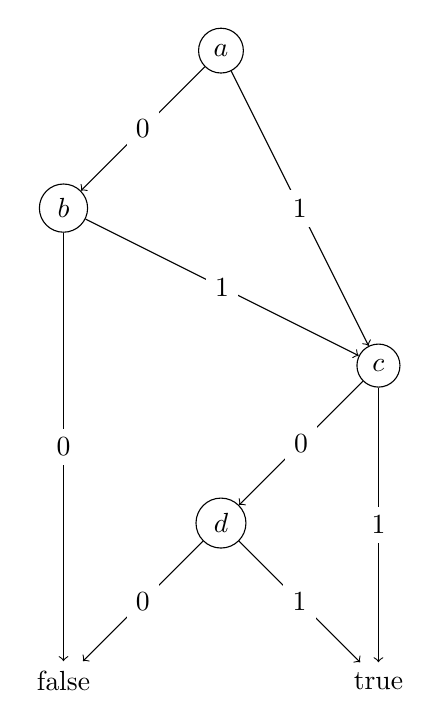
\begin{tikzpicture}[align=center, xscale=2, yscale=2]

\node [circle, draw] (a) at (0, 2) {$a$};
\node [circle, draw] (b) at (-1, 1) {$b$};
\node [circle, draw] (c) at (1, 0) {$c$};
\node [circle, draw] (d) at (0, -1) {$d$};
\node (false) at (-1, -2) {false};
\node (true) at (1, -2) {true};

\draw [->] (a) -- (b) node [midway, fill=white] {0};
\draw [->] (a) -- (c) node [midway, fill=white] {1};
\draw [->] (b) -- (c) node [midway, fill=white] {1};
\draw [->] (b) -- (false) node [midway, fill=white] {0};
\draw [->] (c) -- (true) node [midway, fill=white] {1};
\draw [->] (c) -- (d) node [midway, fill=white] {0};
\draw [->] (d) -- (false) node [midway, fill=white] {0};
\draw [->] (d) -- (true) node [midway, fill=white] {1};

\end{tikzpicture}
\caption{Binary decision diagram for $(a \lor b) \land (c \lor d)$}
\label{fig:bdd}
\end{figure}


\subsection{Data-flow analysis}

The data-flow analysis represents program as a control flow graph where
nodes are blocks of the program and edges represent the flow of
control. Block is a succession of program instructions where control
enters at the beginning of the block, leaves at the end and does not
branch or halt inside the block. The analysis is executed in two steps:
first a set desired facts is compiled, then the set is used for the
analysis itself \cite{Wogerer05-1}. An example of a control flow graph
with corresponding code can be found in figure \ref{fig:dfg}.

This technique is typically used by compilers to optimize the code. It
can help with detecting constant propagation, common subexpression
elimination or redundant operations \cite{Kildall73-1}. However, it is
not powerful enough to provide detailed information that could be used
to prevent runtime errors due to omitting the program semantics by usage
of blocks.

\begin{figure}[ht]
\begin{minipage}{0.3\textwidth}
\begin{lstlisting}
int x = 1;
int i = 0;
do {
    x = x * i;
    i = i + 1;
} while (i < 5);
return x;
\end{lstlisting}
\end{minipage}
\begin{minipage}{0.7\textwidth}
\centering
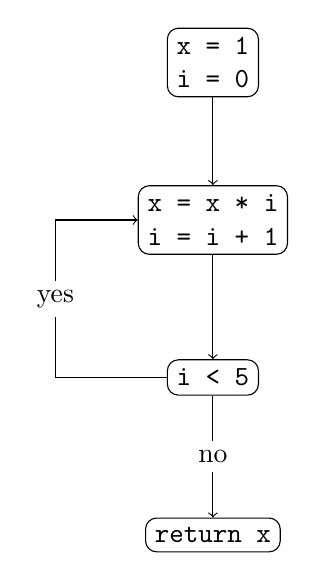
\begin{tikzpicture}[align=center, xscale=2, yscale=2]

\node[block] (init) at (0, 2) {\texttt{x = 1} \\ \texttt{i = 0}};
\node[block] (loop) at (0, 1) {\texttt{x = x * i} \\ \texttt{i = i + 1}};
\node[block] (cond) at (0, 0) {\texttt{i < 5}};
\node[block] (end) at (0, -1) {\texttt{return x}};

\draw [->] (init) -- (loop);
\draw [->] (loop) -- (cond);
\draw [->] (cond) -- (-1, 0) -- node [midway, fill=white] {yes} (-1, 1) -- (loop);
\draw [->] (cond) -- (end) node [midway, fill=white] {no};

\end{tikzpicture}
\end{minipage}
\caption{Data flow graph and corresponding code}
\label{fig:dfg}
\end{figure}


\subsection{Symbolic execution}

The basic idea of symbolic execution is to use symbolic variables instead of
the real ones. For instance, one such usage can be observed in
figure \ref{fig:se}. Throughout the process of symbolic execution
Satisfiability Modulo Theories (SMT) solver checks whether a certain formula
is satisfied \cite{Cadar11-1}.

The main disadvantage of this approach is scalability -- a symbolic
execution of moderately complex program can lead to large number of paths
that need to be checked. That being said, the continuous evolution in
algorithm design and computer performance mitigate this problem.

Symbolic execution is employed by Klee \footnote{\url{http://klee.llvm.org/}}
static analyzer.

\begin{figure}[ht]
\begin{minipage}{0.25\textwidth}
\begin{lstlisting}[numbers=left]
a = a + b;
b = a - b;
a = a - b;
\end{lstlisting}
\end{minipage}
\begin{minipage}{0.75\textwidth}
\begin{tabular}{c|c|c}
line & $a$                       & $b$ \\
\hline
1    & $a + b$                   & $b$ \\
2    & $a + b$                   & $(a + b) - b$ \\
3    & $(a + b) - ((a + b) - b)$ & $(a + b) - b$ \\
\hline \hline
final values & $b$             & $a$ \\
\end{tabular}
\end{minipage}
\caption{Sample code and corresponding symbolic execution}
\label{fig:se}
\end{figure}

\subsection{Abstract interpretation}

A program is represented by set of instructions. When the program is
running, every instruction changes the state of the program. Similarly,
the execution of every instruction depends on the previous state.
The abstract interpretation attempts to eliminate the number of possible
program states by using an abstraction to encapsulate multiple states at
once. It is described in detail in section \ref{sec:abstractinterpretation}.


\chapter{Strings in abstract interpretation}
\label{chap:preliminaries}

This chapter is split into two parts:
first part presents theoretical foundations and basic terms for
abstract interpretation. Strings and their properties are defined in the
second part. Both of these parts support the terminology used throughout
the next chapters.


\section{Abstract interpretation}
\label{sec:abstractinterpretation}

The abstract interpretation falls into the category of software
verification methods by static analysis. It was first defined by P. Cousot
and and R. Cousot in 1977 \cite{CousotCousot77-1}:

\begin{definition}
Abstract interpretation of program consists of using denotations of
computations in some universe of objects to describe computations in
another universe of abstract objects, so that the results of abstract
execution give some informations on the actual computations.
\end{definition}

The key concept here is abstraction. An \textit{abstraction} is a property
of an object that is being analyzed. In figure \ref{fig:abstraction}
there are several abstractions of number 8. This number is positive,
integer, real and rational number. Every one of these abstractions comes
at a cost of precision. The greater the abstraction is the greater is the
loss of precision. Still, an abstraction is often easier to reason about,
mainly in terms of memory -- rather than keeping an enumeration of all
possible values of a number, only an abstraction is kept in memory.

\begin{figure}[ht]
\centering
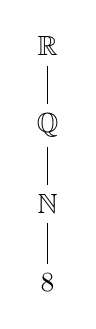
\begin{tikzpicture}[align=center]

\node (real) at (0, 3) {$\mathbb{R}$};
\node (rational) at (0, 2) {$\mathbb{Q}$};
\node (natural) at (0, 1) {$\mathbb{N}$};
\node (eight) at (0, 0) {8};

\draw (real) -- (rational);
\draw (rational) -- (natural);
\draw (natural) -- (eight);

\end{tikzpicture}
\caption{Various abstractions of number 8}
\label{fig:abstraction}
\end{figure}

Number 8 from this example represents a \textit{concrete value}. It is
the value that is used during the actual computation. On the other hand
\textit{abstract value} is the approximation of concrete value used for
abstract interpretation purposes.

Let the set of concrete values $\mathcal{C}$ and set of abstract values $A$,
their members are identified as $C \in \mathcal{C}$ and $a \in A$.

The shift from concrete value to abstraction is done with
\textit{abstraction function}. This function maps a set of concrete values
to abstract value which has properties of interest. It is traditionally
denoted as $\alpha$ \cite{CousotCousot76-1}.

\begin{align*}
\alpha : \mathcal{C} \to A
\end{align*}

For instance, let the abstraction be positive or negative numbers on set of
real numbers $\mathbb{R}$. A few outputs of abstraction function are in
example \ref{ex:abstractionfunc}.

\begin{example}
\label{ex:abstractionfunc}
\begin{align*}
\alpha(A) &=
\begin{cases}
(0) & \text{if } A = \{ 0 \} \\
(+) & \text{if } \forall a \in A : a > 0 \\
(-) & \text{if } \forall a \in A : a < 0 \\
(\pm) & \text{otherwise}
\end{cases} \\
\alpha(\{ -3.4, -1, -17 \}) &= (-) \\
\alpha(\{ 1, 7.35 \}) &= (+) \\
\alpha(\{ -5, 2.7 \}) &= (\pm) \\
\end{align*}
\end{example}

Complementary to the abstraction function is \textit{concretization
function}. It is usually denoted as $\gamma$. It performs a mapping from
abstract value to a set of concrete values. Formally
\cite{CousotCousot76-1}:

\begin{align*}
\gamma : A \to \mathcal{C}
\end{align*}

Following the previous example, the concretization function for abstraction
of positive and negative numbers on $\mathbb{R}$ returns results such as
displayed in example \ref{ex:concretizationfunc}. The function in this
example returns all the values that fall into the intervals of positive
or negative numbers. This property is called \textit{over-approximation}.

\begin{example}
\label{ex:concretizationfunc}
\begin{align*}
\gamma(C) &=
\begin{cases}
\{ 0 \} & \text{if } C = 0 \\
(0, \infty \rangle & \text{if } C = (+) \\
\langle -\infty, 0) & \text{if } C = (-) \\
\langle -\infty, \infty \rangle & \text{otherwise}
\end{cases} \\
\gamma((+)) &= (0, \infty \rangle \\
\gamma((-)) &= \langle -\infty, 0) \\
\gamma((\pm)) &= \langle -\infty, \infty \rangle \\
\end{align*}
\end{example}

Naturally, operations on concrete values need to be somehow transformed
in order to function on abstract values. N\"{a}ive approach to this problem
would be to use the concretization function $\gamma$ to transform abstract
values to concrete values, perform the actual operation and then turn the
concrete values back to abstract using abstraction function $\alpha$.
Unfortunately, such an approach is very computation-demanding. Instead,
concrete operations should be transformed to their ``native'' counterparts
which operate with abstract values directly. An operation that has been
transformed this way is called \textit{abstract operation}.

Consider the abstraction of positive and negative numbers on the set of real
numbers $\mathbb{R}$. The operation of adding $+$ is straightforward for
concrete numbers. However, its matching abstract operation $\oplus$ can
return interesting results. The list of all possible results is in
table \ref{tab:abstractplus}. Note that $(+) \oplus (-) = (\pm)$, because
$2 + (-1) = 1$ and $2 + (-3) = -1$. The $\pm$ sign represents both
positive and negative number since it can not be decided with certainty
whether the result is one or the other. Thus, the result is in this case
imprecise.

\begin{table}[ht]
\centering
\begin{tabular}{c|c|c}
\multicolumn{2}{c|}{$\oplus$} & result \\
\hline
$(+)$ & $(+)$ & $(+)$ \\
$(+)$ & $(-)$ & $(\pm)$ \\
$(-)$ & $(+)$ & $(\pm)$ \\
$(-)$ & $(-)$ & $(-)$ \\
\end{tabular}
\caption{Abstract operation $\oplus$ semantics}
\label{tab:abstractplus}
\end{table}

That being said, the loss of precision does not occur always. Multiplication
of two abstract values $\otimes$ always returns precise result regardless
of whether the values are abstract or concrete. The table
\ref{tab:abstractmult} shows all possible situations for this operation.
Notice the lack of precision loss.

\begin{table}[ht]
\centering
\begin{tabular}{c|c|c}
\multicolumn{2}{c|}{$\otimes$} & result \\
\hline
$(+)$ & $(+)$ & $(+)$ \\
$(+)$ & $(-)$ & $(-)$ \\
$(-)$ & $(+)$ & $(-)$ \\
$(-)$ & $(-)$ & $(+)$ \\
\end{tabular}
\caption{Abstract operation $\otimes$ semantics}
\label{tab:abstractmult}
\end{table}


For the purpose of comparing two values some sort of element ordering and
associated terms need to be defined \cite{Burris81-1}:

\begin{definition}
A partial order $\leq$ is binary relation defined on set $A$, when following
rules hold:

\begin{align}
\forall a \in A &: a \leq a \label{eq:refl} \\
\forall a, b \in A &: a \leq b \land b \leq a \Rightarrow a = b \label{eq:antisym} \\
\forall a, b, c \in A &: a \leq b \land b \leq c \Rightarrow a \leq c \label{eq:trans}
\end{align}

These rules are also known as \textit{reflexivity} (\ref{eq:refl}),
\textit{antisymmetry} (\ref{eq:antisym}) and \textit{transitivity} (\ref{eq:trans}).

Partially ordered set is denoted as $\langle A, \leq \rangle$
\end{definition}

\begin{example}
$\langle \mathbb{N}, \leq \rangle$ is partially ordered set.
\end{example}

\begin{definition}
Let $\langle A, \leq \rangle$ be a partially ordered set.

\begin{itemize}

\item element $u \in A$ is an \textit{upper bound} of $S \subseteq A$ if
$\forall s \in S : s \leq u$

\item element $l \in A$ is a \textit{lower bound} of $S \subseteq A$ if
$\forall s \in S : l \leq s$

\item element $u \in A$ is a \textit{least upper bound} of $S \subseteq A$
if $\forall u' \in A : (\forall s \in S : s \leq u') \Rightarrow u \leq u'$

\item element $l \in A$ is a \textit{greatest lower bound} of $S \subseteq A$
if $\forall l' \in A : (\forall s \in S : l' \leq s) \Rightarrow l' \leq l$

\end{itemize}

The least upper bound is often called \textit{supremum} (denoted as $\sup$)
or \textit{join} (denoted as $\lor$). The greatest lower bound is also
called \textit{infimum} (denoted as $\inf$) or \textit{meet} (denoted as
$\land$).
\end{definition}

\begin{example}
Let $A = \{ 1, 2, 3 \}$ ordered by operation $\leq$ then
$\sup A = 3, \inf A = 1$.
\end{example}

Analyzed values need to be described by a mathematical structure that is
compliant with requirements posed by abstract interpretation. Ordinarily,
a \textit{lattice} is used in this context. It is defined as
\cite{Burris81-1}:

\begin{definition}
A lattice is tuple $L = \langle A, \leq \rangle$, where:

\begin{itemize}
\item $A$ is a set of all elements
\item $\leq$ is partial order on $A$
\item $\forall a, b \in A : \sup \{ a, b \} \in A \land \inf \{ a, b \} \in A$
\end{itemize}
\end{definition}

Frequently, join and meet operations are extracted to emphasize their
special position within the lattice --
$L = \langle A, \leq, \land, \lor \rangle$.
A lattice is typically displayed as \textit{Hasse diagram}. An example
of such diagram for $A = \{ 1, 2, 3\}$ ordered by operation set inclusion
$\subseteq$ is displayed in figure \ref{fig:concretedomain}.

\begin{definition}
A complete lattice is tuple $L = \langle A, \leq, \land, \lor, \bot, \top \rangle$
where $\forall S \subseteq A$ :

\begin{itemize}
\item least upper bound $\lor$ of $S$ exists
\item greatest lower bound $\land$ of $S$ exists
\end{itemize}

Elements $\bot$ and $\top$ denote $\sup$ and $\inf$ of $A$ respectively.
\end{definition}

\begin{example}
Lattice $\langle \mathcal{P}(\mathbb{N}), \subseteq, \cap, \cup, \emptyset, \mathbb{N} \rangle$
is a complete lattice.
\end{example}

Concrete values of program interpretation are organized in \textit{concrete
domain}. Formally, the concrete domain is a complete lattice $L$ on set
$A$ \cite{Constantini11-1}:

\begin{align*}
L = \langle \mathcal{P} (A), \subseteq, \emptyset, A, \cap, \cup \rangle
\end{align*}

where $\mathcal{P} (A)$ is power set of $A$. An example of such lattice
for set $A = \{ 1, 2, 3 \}$ can be found in figure \ref{fig:concretedomain}.

\begin{figure}[ht]
\centering
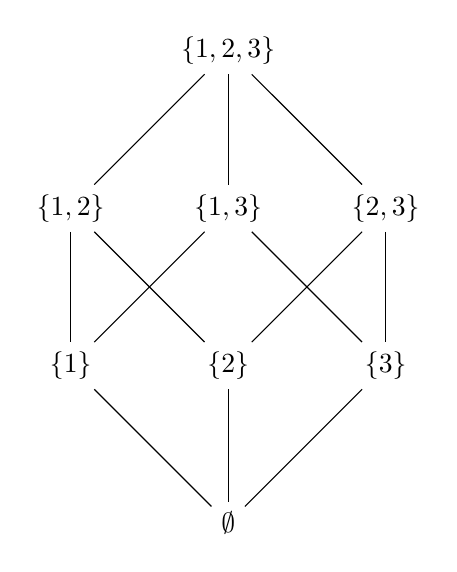
\begin{tikzpicture}[align=center, xscale=2, yscale=2]

\node (123) at (0, 3) {$\{ 1, 2, 3 \}$};
\node (12) at (-1, 2) {$\{ 1, 2 \}$};
\node (13) at (0, 2) {$\{ 1, 3 \}$};
\node (23) at (1, 2) {$\{ 2, 3 \}$};
\node (1) at (-1, 1) {$\{ 1 \}$};
\node (2) at (0, 1) {$\{ 2 \}$};
\node (3) at (1, 1) {$\{ 3 \}$};
\node (empty) at (0, 0) {$\emptyset$};

\draw (123) -- (12);
\draw (123) -- (13);
\draw (123) -- (23);
\draw (12) -- (1);
\draw (12) -- (2);
\draw (13) -- (1);
\draw (13) -- (3);
\draw (23) -- (2);
\draw (23) -- (3);
\draw (1) -- (empty);
\draw (2) -- (empty);
\draw (3) -- (empty);

\end{tikzpicture}
\caption{Concrete domain for set $\{ 1, 2, 3 \}$}
\label{fig:concretedomain}
\end{figure}

Abstract properties are encoded in modules with data structures called
\textit{abstract domain}. This module is a set of all abstract values
for given abstraction. Formally, abstract domain forms a complete
lattice $L'$ \cite{Constantini11-1}:

\begin{align*}
L' = \langle \bar{A}, \sqsubseteq, \bot, \top, \sqcup, \sqcap  \rangle
\end{align*}

Intuitively, the abstract domain encapsulates multiple concrete states of
program execution. Consider the abstraction of positive and negative
numbers on set of real numbers $\mathbb{R}$. The abstract domain for this
abstraction is displayed in figure \ref{fig:abstractdomain}.

\begin{figure}[ht]
\centering
\begin{tikzpicture}[align=center]

\node (top) at (0, 3) {$\top$};
\node (negative) at (-1, 2) {$(-)$};
\node (positive) at (1, 2) {$(+)$};
\node (zero) at (0, 1) {$0$};
\node (bottom) at (0, 0) {$\bot$};

\draw (top) -- (negative);
\draw (top) -- (positive);
\draw (negative) -- (zero);
\draw (positive) -- (zero);
\draw (zero) -- (bottom);

\end{tikzpicture}
\caption{Abstract domain for positive and negative numbers on $\mathbb{R}$}
\label{fig:abstractdomain}
\end{figure}

The relationship between concretization and abstraction is described by
\textit{Galois connection} \cite{CousotCousot92-4}:

\begin{definition}
If $L$ and $L'$ are lattices the $\langle \alpha, \gamma \rangle$ is
a Galois connection, written $L \galois{\alpha}{\gamma} L'$ if and only if
$\alpha \in L \to L'$ and $\gamma \in L' \to L$ are functions such that:

\begin{align*}
\forall x \in L, y' \in L': (\alpha(x) \leq y') \iff (x \leq \gamma(y'))
\end{align*}
\end{definition}

\begin{example}
Consider the set of real numbers $\mathbb{R}$, abstraction function
$\alpha$ from example \ref{ex:abstractionfunc} and concretization function
$\gamma$ from example \ref{ex:concretizationfunc}.
$\langle \alpha, \gamma \rangle$ forms Galois connection.
\end{example}

Suppose a function $f: L \to L$ then $l$ is a \textit{fixed point}
if $f(l) = l$. A fixed point can be achieved by using an iterative process
such as $f_n(l) = f(f( \dots f(\bot) \dots ))$. Unfortunately, this process
does not necessarily have to converge to the fixed point or terminate.
Because of that, an approximation for iteration must be used. Termination
can be achieved via \textit{widening} operator. As an example, consider a
computation which has not reached the fixed point after 10 iterations.
To terminate the process, the value is set to $\top$ hence the fixed point
is reached -- $f(\top) = \top$. This approach is simple to implement but
results obtained this way are very imprecise.

To conclude, the abstract interpretation attempts to achieve fixed point of
abstract values by taking advantage of partial ordering of these values.
While iterating through the program it uses abstract operations on abstract
domains to obtain new abstract values until the fixed point is reached.
Abstract operations move the abstract values ``upwards'' in their respective
domain lattices.

Abstract interpretation should ideally be sound, complete and should
terminate \cite{aiaa10}. As previously shown, termination can be achieved by
using widening. Soundness of interpretation means that any property proved
in abstraction is valid in concrete. Completeness means that property in
the concrete is valid in abstract. In reality, abstracts interpreter are
designed to be sound and to terminate, but they are incomplete. This is
a result of the undecidability of Halting problem as described in
section \ref{sec:softwarequality}.

This method promises better scalability when compared to other
methods such as model checking or symbolic execution. It tries to achieve
this through appropriate abstraction choice. In fact, the choice of suitable
abstraction is crucial in this promise. Moreover, abstract interpretation
provides a theoretical framework that unifies other static analysis
approaches such as data-flow analysis \cite{CousotCousot77-1} or model
checking \cite{CousotCousot99-1}.


\section{Strings}
\label{sec:strings}

Strings of characters are widely employed in software engineering. They
represent basic building blocks in dynamically typed languages such as
Python, Ruby or Perl. Their usages include expressions of values,
arguments, commands or even whole pieces of code. Strings are frequently
used during generating an output such as XML file or processing an input
in text form. The format of the processed string is often verified by
another part of the system which takes this string as an input, for
instance the format of a SQL query is verified by SQL server processor
which can cause unexpected errors. Moreover, a user might supply a
malicious input when deliberately trying to cause similar effect.
Therefore, it is useful to know how string is formatted and manipulated
during the execution of a program.

The following definitions are describe strings and their properties
formally \cite{Kozen97-1}:

\begin{itemize}

\item An \textit{alphabet} is any finite set. For example an alphabet for
binary numbers is $\{0, 1\}$. It is typically denoted as $\Sigma$. Elements
of alphabet are called \textit{symbols} or \textit{letters} and are denoted
by $a, b, c, \dots$.

\item A \textit{string} over $\Sigma$ is any finite sequence of symbols of
$\Sigma$. For $\Sigma = \{a, b\}$ an example of string is $aabab$. Strings
are denoted by $x, y, z, \dots$.

\item The \textit{length} of a string $x$ is the number of symbols in $x$.
It is denoted as $|x|$. For example, $|aabab| = 5$.

\item \textit{Empty string} is a string with length of 0. It is also called
\textit{null string} and is denoted by $\varepsilon$. Formally,
$|\varepsilon| = 0$.

\item \textit{Concatenation} is an operation which takes two strings $x$
and $y$ and chains them together to form a new string $xy$. It is
associative operation but it not commutative. Empty string $\varepsilon$ is
identity for concatenation. The length of resulting string is a sum of
lengths of concatenated strings.

\begin{align*}
(xy)z &= x(yz) \\
xy &\neq yx \\
\varepsilon x = x \varepsilon &= x \\
|xy| &= |x| + |y|
\end{align*}

\item A \textit{prefix} of a string $x$ is a string $y$ for which there
exists a string $z$ such that $x = yz$. The empty string $\varepsilon$ is
a prefix of every string. String $aaba$ is a prefix of $aababb$. A prefix
$y$ of $x$ is a \textit{proper} prefix of $x$ when $y \neq \varepsilon$ and
$y \neq x$.

\item A \textit{suffix} of a string $x$ is a string $z$ for which there
exists a string $y$ such that $x = yz$. The empty string $\varepsilon$ is
a suffix of every string. String $babb$ is a suffix of $aababb$. A suffix
$z$ of $x$ is a \textit{proper} suffix of $x$ when $z \neq \varepsilon$ and
$z \neq x$.

\end{itemize}

In \texttt{C} programming language strings are separated from the rest of
the code by pair of \texttt{"} (double quote) characters. Internally,
they represent a chunk of memory structurally similar to array. In fact,
string is a specific type of array. Generally, an array can contain any
type of data given all the array items have the same type \footnote{In some
languages members of array do not have to be uniformly typed.} and for
string that data type happens to be \texttt{char}. The end of the string is
determined by a special character \texttt{'\textbackslash0'} called NUL.
Strings terminated by such character are usually called null-terminated
strings.

Obviously, strings and arrays are related to each other quite tightly.
Both of them serve as sets of values sequentially stored in memory.
Nonetheless, there is a difference in the information value they represent.
For example, in an array of integers the information value is uniformly
distributed -- every number in the array carries the same weight. On the
other hand, symbols of string do not carry a lot of information just by
themselves. Having three characters \texttt{'v'}, \texttt{'a'} and
\texttt{'r'} separately does not mean a lot, but together they form
a \texttt{"var"} string which might tell a programmer that variable
declaration follows.

The versatility of strings makes it difficult to analyze them in general.
Intuitively, one can feel there is a difference when trying to analyze
string containing an XML document and string containing SQL query. They
have different properties of interest and they both need to be formatted
differently.


\chapter{Design of string abstractions}
\label{chap:design}

This chapter describes strings and three approaches that have been designed
to analyze strings within abstract interpretation framework. Strings play
an important role in day-to-day computer programming. Nowadays, they are
an essential part of every major programming language.


\section{String abstract domains}

The primary goal of domains described in following sections is to
abstract strings so that they provide useful informations about file
paths. Normally, in UNIX-like operating systems such as Linux or Mac OS
the path is represented by a string containing slash \texttt{'/'} characters
and names of folders or files in between them. An example of such path could
be \texttt{"/var/lib/dhcpcd"}.

As per the definition of abstract domain from section
\ref{sec:abstractinterpretation} the members of complete lattice need to be
specified for every suggested domain:

\begin{itemize}

\item set $A$ contains abstract values of particular set (prefixes,
suffixes, tries)

\item partial ordering $\leq$ of abstract values in abstract domain

\item least upper bound $\sqcap$ for every pair of abstract values

\item greater lower bound $\sqcup$ for every pair of abstract values

\item top element $\top$

\item bottom element $\bot$

\end{itemize}

Besides that, the operations specific to particular domain need to be
defined. In this case these are based on functions available to programmer.
Obviously, the C standard library provides numerous functions that operate
on strings, but for the purposes of this work concatenation and
substring functions will suffice. These function have been chosen because
they modify string. They are denoted as \textit{concat} and
\textit{substr} respectively.

The \textit{concat} function has two arguments -- strings that need to be
concatenated. The function follows the semantics of concatenation
operation described in section \ref{sec:strings} and returns these two
strings chained together as one. For instance,
$\textit{concat}(\texttt{"geo"}, \texttt{"logy"})$ yields \texttt{"geology"}.

The \textit{substr} function takes three arguments: a string $x$ and two
natural numbers $i$ and $j$ assuming $i < j$. The function returns a
substring of string $x$ from the $i$-th to the $j$-th symbol of the string.
Note that strings are indexed the same way as arrays -- $x[0]$ is the first
symbol of $x$, $x[1]$ is the second and so on. As an example consider the
function $\textit{substr}(1, 4, \texttt{"automatic"})$ which returns
\texttt{"utom"}.


\section{Prefix abstract domain}

The first of the designed abstract domains is the one that approximates
a string by its prefix. It is based of works of Giulia Constantini,
Pietro Ferrara and Agostino Cortesi \cite{Constantini11-1}. This domain
is has simple semantics, thus it provides a good introduction into the
designed abstract domains.

The abstraction used in this case is string prefix as defined in section
\ref{sec:strings}. Common notation for prefix is $abc*$ where $abc$
represents symbols of prefix and $*$ stands for any string, $\varepsilon$
included. The asterisk is present in prefix all the time so it can be
omitted from this notation.

Partial ordering $\leq$ on this domain is defined as:

\begin{align*}
x \leq y \Leftrightarrow
  x = \bot \lor (\forall i \in [0, |y| - 1] :
  |y| \leq |x| \land y[i] = x[i])
\end{align*}

where $x$ and $y$ are abstract values representing string prefixes.

Intuitively, prefixes are ordered in a lattice by their length. Prefix
$x$ is smaller than string $y$ if $y$ is a
prefix of $x$ or $x$ is the bottom of the domain $\bot$.
The length of string abstract values decreases as prefixes are closer to
the top element $\top$. The situation is demonstrated in figure
\ref{fig:prefixlattice}.

\begin{figure}[ht]
\centering
\begin{tikzpicture}[align=center]

\node (top) at (0, 3) {$\top$};
\node (s) at (0, 2) {s};
\node (sa) at (-2, 1) {sa};
\node (su) at (2, 1) {su};
\node (sax) at (-3, 0) {sax};
\node (sap) at (-1, 0) {sap};
\node (sup) at (1, 0) {sup};
\node (sud) at (3, 0) {sud};
\node (bottom) at (0, -1) {$\bot$};

\draw (top) -- (s);
\draw (s) -- (sa);
\draw (s) -- (su);
\draw (sa) -- (sax);
\draw (sa) -- (sap);
\draw (su) -- (sup);
\draw (su) -- (sud);
\draw (sax) -- (bottom);
\draw (sap) -- (bottom);
\draw (sup) -- (bottom);
\draw (sud) -- (bottom);

\end{tikzpicture}
\caption{Prefix abstract domain}
\label{fig:prefixlattice}
\end{figure}

The least upper bound operator $\sqcap$ is defined as:

\begin{align*}
\sqcap (x, y) =
\begin{cases}
z & \text{where } z
  = \textit{prefix}(x, y) \\
\top       & \text{otherwise}
\end{cases}
\end{align*}

where function $\textit{prefix}(x, y)$ returns the
longest common prefix of strings $x$ and $y$. For
example, $\textit{prefix}(\texttt{"capture"}, \texttt{"caption"})$ returns
\texttt{"capt"} and for $\textit{prefix}(\texttt{"house"}, \texttt{"car"})$
returns $\varepsilon$.

Simply put, the least upper bound of two strings $x$ and $y$
is the longest common prefix of these strings. If there is
none, the upper bound is the top element of the lattice $\top$.

In a similar fashion, the greater lower bound operator $\sqcup$ is defined
by:

\begin{align*}
\sqcup (x, y) =
\begin{cases}
x    & \text{if } x \leq y \\
y    & \text{if } y \leq x \\
\bot & \text{otherwise}
\end{cases}
\end{align*}

The greater lower bound is the smaller of the two elements and if none
of them is smaller then it is the bottom element $\bot$.

The semantics for \textit{concat} operation is defined as:

\begin{align*}
\textit{concat}(x, y) = x
\end{align*}

where $x$ and $y$ are string prefixes. The \textit{concat} operation of two
prefixes returns the first of the concatenated prefixes since it is the
longest prefix that is surely included in resulting string.

The \textit{substr} operations semantics is defined by:

\begin{align*}
\textit{substr}(i, j, x) =
\begin{cases}
x[i] \dots x[j - 1]   & \text{if } j \leq |x| \\
x[i] \dots x[|x| - 1] & \text{if } j > |x| \land i < |x| \\
\top                  & \text{otherwise}
\end{cases}
\end{align*}

The situation for substring function is not so straightforward.
The \textit{substr} function returns substring from $i$-th to $j$-th symbol
when index $j$ is less than the length of $x$, it returns symbols from
$i$-th index to the end of $x$ if $i$ is less the length of $x$ but $j$
is greater than the string length and it returns $\top$ top element in
all other cases.


\section{Suffix abstract domain}

The second domain is complementary to the domain approximating using
prefixes. It was presented in the same paper \cite{Constantini11-1} as the
prefix domain. It is relatively simple as well.

Abstract values for this domain are represented by string suffixes.
The notation chosen for suffixes is $*abc$ where $abc$ are symbols of
suffix and $*$ any string. The asterisk is left out since it is always
there.

Partial order $\leq$ for suffixes $x$ and $y$ is:

\begin{align*}
x \leq y \Leftrightarrow
  x = \bot \lor (\forall i \in [0, |y| - 1] : |y| \leq |x| \land
    y[i] = x[i + |x| - |y|])
\end{align*}

For better illustration, the figure \ref{fig:suffixlattice} shows an
example of suffix abstract domain with such order.

\begin{figure}[h]
\centering
\begin{tikzpicture}[align=center]

\node (top) at (0, 3) {$\top$};
\node (n) at (0, 2) {n};
\node (on) at (-2, 1) {on};
\node (un) at (2, 1) {un};
\node (ion) at (-3, 0) {ion};
\node (ton) at (-1, 0) {ton};
\node (sun) at (1, 0) {sun};
\node (fun) at (3, 0) {fun};
\node (bottom) at (0, -1) {$\bot$};

\draw (top) -- (n);
\draw (n) -- (on);
\draw (n) -- (un);
\draw (on) -- (ion);
\draw (on) -- (ton);
\draw (un) -- (sun);
\draw (un) -- (fun);
\draw (ion) -- (bottom);
\draw (ton) -- (bottom);
\draw (sun) -- (bottom);
\draw (fun) -- (bottom);

\end{tikzpicture}
\caption{Suffix abstract domain}
\label{fig:suffixlattice}
\end{figure}

The least upper bound $\sqcap$ is:

\begin{align*}
\sqcap (x, y) =
\begin{cases}
z    & \text{where } z = \textit{suffix}(x,  y) \\
\top & \text{otherwise}
\end{cases}
\end{align*}

where function \textit{suffix} returns the longest common suffix of the
two strings $x$ and $y$. If these strings have common suffix then the least
upper bound is their longest common suffix. Otherwise it is the top
element $\top$.

The greatest lower bound is defined as:

\begin{align*}
\sqcup (x, y) =
\begin{cases}
x    & \text{if } x \leq y \\
y    & \text{if } y \leq x \\
\bot & \text{otherwise}
\end{cases}
\end{align*}

If it is possible to compare the two strings, then it is the smaller of the
two. It is the bottom element $\bot$ for all other cases.

The \textit{concat} operation for suffix domain is the second of the
concatenated strings:

\begin{align*}
\textit{concat}(x, y) = y
\end{align*}

The \textit{substr} operation is unusually simple:

\begin{align*}
\textit{substr}(i, j, x) = \top
\end{align*}

It returns the top element $\top$ for all the possible inputs, because
it is impossible to tell whether indexes $i$ and $j$ are within the
boundaries of the suffix.

An example of the domain usage could be filtering files or directories
based on their extensions.


\section{Trie abstract domain}

Trie abstract domain approximates string as \textit{trie} data structure.
The name trie comes from word ``retrieval'' as in information retrieval. It
is a tree-like data structure where every node represents a set of all keys
that begin a certain sequence of symbols -- prefix. Trie is especially useful
for searching purposes because it provides good tradeoff between the memory
consumption and performance.

In order to preserve memory space, the trie can be compressed. Nodes can
contain whole substrings, not just symbols of the string. This optimization
should reduce the number of trie nodes. As a result of this optimization
every node that is not leaf has at least two children. This is the type of
trie which will be used throughout this thesis. An example of a trie
representing strings \texttt{"great"}, \texttt{"growth"} and \texttt{"good"}
can be found in figure \ref{fig:trie}. Children of each node are
lexicographically ordered.

\begin{figure}[ht]
\centering
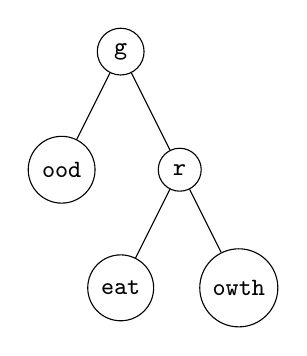
\begin{tikzpicture}[font=\small]

\node [circle, draw] (g) {\texttt{g}}
  child {node [circle, draw] (ood) {\texttt{ood}}}
  child {node [circle, draw] (r) {\texttt{r}}
    child {node [circle, draw] (eat) {\texttt{eat}}}
    child {node [circle, draw] (owth) {\texttt{owth}}}
  };

\path (g) -- (r);
\path (g) -- (ood);
\path (r) -- (eat);
\path (r) -- (owth);

\end{tikzpicture}
\caption{Trie representing strings \texttt{"great"}, \texttt{"growth"} and
  \texttt{"good"}}
\label{fig:trie}
\end{figure}

This domain provides better precision than prefix or suffix, but it is more
resource-demanding in terms of both the space it occupies and the time it
takes to perform operations on it.

Suppose $\mathcal{x}$ denote a trie. Notation $|\mathcal{x}|$ means a number of
strings represented by trie and $\mathcal{x}[i]$ is $i$-th string of the trie
starting from 0. Let $\mathcal{x}$ be the trie from figure \ref{fig:trie}.
In this case $|\mathcal{x}| = 3$ and $\mathcal{x}[0] = \texttt{"good"},
\mathcal{x}[1] = \texttt{"great"}, \mathcal{x}[2] = \texttt{"growth"}$.
Note that the way a string is divided between nodes of the trie does not
matter. 

The partial ordering for tries $\mathcal{x}$ and $\mathcal{y}$ is defined as:

\begin{align*}
x \leq y \Leftrightarrow
  x = \bot \lor (\forall i \in [0, |x| - 1] : x[i] \in y)
\end{align*}

The trie $\mathcal{x}$ is smaller than trie $\mathcal{y}$ if all strings
represented by $\mathcal{x}$ are also present in $\mathcal{y}$ or if trie
$\mathcal{x}$ is the bottom element $\bot$ of lattice. The number of nodes
increases over the course of interpretation as elements of lattice get
closer to the top $\top$. An example of a lattice with such order is shown
in figure \ref{fig:trielattice}.

\begin{figure}[ht]
\centering
\begin{tikzpicture}[xscale=3, yscale=3]

\node (top) at (0, 4) {$\top$};
\node [block,draw] (stopepuper) at (0, 3) {
  \begin{tikzpicture}[xscale=0.5, yscale=0.5, font=\tiny]
    \node{s}
      child {node {t}
        child {node {op}}
        child {node {ep}}
      }
      child {node {uper}}
    ;
  \end{tikzpicture}
};
\node [block,draw] (stopep) at (-1, 2) {
  \begin{tikzpicture}[xscale=0.5, yscale=0.5, font=\tiny]
    \node{st}
      child {node {op}}
      child {node {ep}}
    ;
  \end{tikzpicture}
};
\node [block, draw] (stopuper) at (0, 2) {
  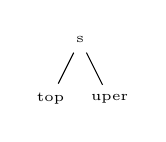
\begin{tikzpicture}[xscale=0.5, yscale=0.5, font=\tiny]
    \node{s}
      child {node {top}}
      child {node {uper}}
    ;
  \end{tikzpicture}
};
\node [block, draw] (stepuper) at (1, 2) {
  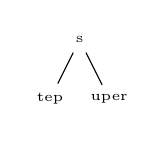
\begin{tikzpicture}[xscale=0.5, yscale=0.5, font=\tiny]
    \node{s}
      child {node {tep}}
      child {node {uper}}
    ;
  \end{tikzpicture}
};
\node [block, draw] (stop) at (-1, 1) {stop};
\node [block, draw] (step) at (0, 1) {step};
\node [block, draw] (super) at (1, 1) {super};
\node (bottom) at (0, 0) {$\bot$};

\draw (top) -- (stopepuper);
\draw (stopepuper) -- (stopep);
\draw (stopepuper) -- (stopuper);
\draw (stopepuper) -- (stepuper);
\draw (stopep) -- (stop);
\draw (stopep) -- (step);
\draw (stopuper) -- (stop);
\draw (stopuper) -- (super);
\draw (stepuper) -- (super);
\draw (stepuper) -- (step);
\draw (stop) -- (bottom);
\draw (step) -- (bottom);
\draw (super) -- (bottom);
  
\end{tikzpicture}
\caption{Trie abstract domain}
\label{fig:trielattice}
\end{figure}

The least upper bound $\sqcap$ is defined as:

\begin{align*}
TODO
\end{align*}

The greatest lower bound $\sqcup$ is defined as:

\begin{align*}
TODO
\end{align*}



\section{Other existing string domains}
\label{sec:otherstringdomains}

TODO


\chapter{Implementation of string abstractions}
\label{chap:implementation}

Abstract domains designed in chapter \ref{chap:design} are applied in the
context of \texttt{canal} abstract interpreter. First part describes the
architecture of the interpreter. The rest of the chapter deals with the
implementation of individual domains.


\section{\texttt{canal}}

Following the project README file \cite{Klic12-1}, the \texttt{canal}
abstract interpreter is a static analysis tool designed to analyze behavior
of application programs written in C programming language. It focuses
on scalability for large programs and handling of real-world source code.

It is divided into three parts:

\begin{description}

\item[Abstract domains] \hfill \\
These modules cover semantic choices, data
structures, algorithmic aspects and implementation details concerning
analysis. Canal contains abstract domains for integers, floating point
numbers, arrays and strings.

\item[Interpreter] \hfill \\
It iterates through the source code until the analysis
is finished. It manages the state of program analysis consisting of
abstract values.

\item[Operations] \hfill \\
They manage translations of program instructions to
abstract operations defined as part of abstract domains. Interpreter uses
operations to update abstract values stored in analysis state.

\end{description}

The tool is utilizes LLVM compiler infrastructure. The infrastructure
provides a front-end called Clang that contains compilers for C, C++,
Objective C and Objective C++ capable of emitting LLVM intermediate
representation. The intermediate representation is a platform independent
representation of program that is suitable for static analysis.
The representation is static single assignment representation that provides
type safety, low-level operations, flexibility and the capability to
represent ``all'' high-level languages cleanly \cite{llvm13-1}. It is similar
to assembly language which is human-readable, see an example in
listing \ref{lst:llvmir}. There are other static analysis tools that leverage
the LLVM intermediate representation, namely Klee.

\begin{lstlisting}[
    caption={LLVM intermediate representation},
    label=lst:llvmir
]

    %Z = add i32 %X, %Y

\end{lstlisting}

The whole process of analysis by \texttt{canal} is performed in following
steps:

\begin{enumerate}

\item compilation of a program that is being analyzed into the LLVM
intermediate representation

\item loading of compiled program into the interpreter and initialization
with abstract domains

\item interpretation of loaded program with abstract operations on the
domains

\end{enumerate}

Abstract interpreter itself is implemented in C++. It can be compiled with
g++ compiler from the GNU Compiler Collection.

\texttt{canal} comes with command line tool which allows to step through
the execution of interpretation and inspect variables. In that aspect it
is similar to \texttt{gdb}, a popular GNU debugger project for various
languages \footnote{\url{http://www.gnu.org/software/gdb/}}.

The project is relatively young and as of this moment is in its experimental
stage. That being said, a few programs from GNU core utilities project
\footnote{\url{http://www.gnu.org/software/coreutils/}} have been
successfully analyzed by interpreter.


\section{Domain interface in \texttt{canal}}

Since \texttt{canal} abstract interpreter is implemented in C++ it enables
the usage of classes. Every domain in it corresponds to single class and
operations on the domain are implemented as methods of the particular class.
Most of the operations are domain-specific, but there are a few methods
that are universally required to be implemented in order for abstract
values to form a lattice.

Universal methods are enforced by inheriting from \texttt{Domain} class,
which provides their type definitions. These methods are:

\begin{itemize}

\item join

\item meet

\item equality -- this operation verifies that two abstract values are the same

\item inclusion --

\item set top -- sets the abstract value to top $\top$

\item set bottom -- sets the abstract value to bottom $\bot$

\item is top -- check if the abstract value is top $\top$

\item is bottom -- check if the abstract value is bottom $\bot$

\end{itemize}


\section{String prefix}

The prefix of a string is internally represented by standard \texttt{string}
container.

TODO


\section{String suffix}

TODO

\section{String trie}

TODO

\chapter{Conclusion}
\label{chap:conclusion}

This thesis has described quality evaluation techniques used in software
engineering. Software verification by static analysis has been defined.
Several examples of methods employing static analysis have been given to
illustrate the application of this technique. Definitions for other methods
such as software validation or dynamic analysis have been supplied as well.
Compelling arguments have been given for each of these approaches and their
limitations have been shown here.

Then, a detailed description of abstract interpretation framework
along with definitions regarding strings. Descriptions are given on both
formal and intuitive levels. This part specifies terms and language used
throughout the design and implementation segments of the work.

The core of the thesis is the design of three abstract domains
approximating strings. The semantics of all properties and operations
have been described and demonstrative examples have been shown in both
graphical and textual form. Domains using string prefix and suffix
closely follow their description as given by Costantini, Ferrara and
Cortesi \cite{Constantini11-1}. The domain using tries as a representation
of string has been created as part of this section.

Three designed string abstract domains have been implemented in context of
the \texttt{canal} abstract interpreter. They have all been covered with
unit tests for better maintainability and understanding of the code.
Implementation closely follows the style defined by the project. This
part of the thesis serves as a technical report regarding implementation
details and decision that have been made during the course of this work.

The contributions of this thesis are:

\begin{itemize}

\item design of the trie abstract domain

\item implementation of abstract domains approximating strings by its
prefix, suffix and trie

\end{itemize}

The trie abstract domain has not been used anywhere else other than
\texttt{canal}. It is the proposition made to improve the precision of the
other two domains. The implementation of the three designed domains is
their first open-source implementation. This creates an opportunity for
community to get involved and improve both design and implementation of this
solution.

Future work may include improving the precision of string analysis by
implementing other string domains. A few examples have been mentioned
in \ref{sec:otherstringdomains}. Also, new domains for strings can be
proposed where properties other than file paths will be considered. However,
one needs to keep in mind that every abstract domain is a tradeoff between
implementation difficulty, precision and performance.

%% Lists of tables and figures, glossary, etc.
%\printindex
%\printglossary
%\listoffigures
%\listoftables

%% Bibliography
\renewcommand*{\bibname}{\chapter{Bibliography}\vspace{-1em}}
\begin{thebibliography}{99}

\bibitem{CousotCousot77-1}
P{.} Cousot and R{.}Cousot.
\newblock Abstract interpretation: a unified lattice model for static
  analysis of programs by construction or approximation of fixpoints.
\newblock In \emph{Conference Record of the Fourth Annual ACM
  SIGPLAN-SIGACT Symposium on Principles of Programming Languages},
  pages 238--252, Los Angeles, California, 1977. ACM Press, New York,
  NY, USA.

\bibitem{Cousot00-1}
P{.} Cousot.
\newblock Abstract interpretation based formal methods and future
  challenges.
\newblock In \emph{Informatics - 10 Years Back, 10 Years Ahead},
  volume 2000 of LNCS, pages 138--156. Springer, 2000.

\bibitem{Moore65-1}
G{.} E{.} Moore.
\newblock Cramming more components onto integrated circuits.
\newblock In \emph{Electronics}, volume 38, number 8, pages 114--117. 1965.

\bibitem{EmanuelssonNilsson08-1}
P{.} Emanuelsson, U{.} Nilsson.
\newblock A comparative study of industrial static analysis tools (extended
  version).
\newblock In \emph{Electronic Notes in Theoretical Computer Science},
  volume 217, pages 5--21. 2008.

\bibitem{iso9000-2000}
\newblock ISO 9000:2000 standard.
\newblock Available at \url{https://www.iso.org/obp/ui/#iso:std:iso:9000:ed-3:v1:en}
  (May 2013).

\bibitem{Ernst03-1}
M{.} D{.} Ernst.
\newblock Static and dynamic analysis: Synergy and duality.
\newblock In \emph{Workshop on Dynamic Analysis}, pages 24--27. 2003.

\bibitem{Woodcock09-1}
J{.} Woodcock, P{.} G{.} Larsen, J{.} Bicarregui and J{.} S{.} Fitzgerald.
\newblock Formal methods: Practise and experience.
\newblock In \emph{ACM Computing Surveys}. 2009.

\bibitem{Turing36-1}
A{.} Turing.
\newblock On computable numbers, with an application to the
  Entscheidungsproblem.
\newblock In \emph{Proceedings of the London Mathematical Society},
  pages 230--265. 1936.

\bibitem{Sipser06-1}
M{.} Sipser.
\newblock Introduction to the Theory of Computation (Second Edition).
\newblock Thomson Course Technology, 2006.

\bibitem{Kozen97-1}
D{.} Kozen.
\newblock Automata and Computability.
\newblock Springer, 1997.

\bibitem{Chess04-1}
B{.} Chess, G{.} McGraw.
\newblock Static Analysis for Security.
\newblock In \emph{Security and Privacy, IEEE}, volume 2, number 6,
  pages 76--79, 2004.

\bibitem{Clarke99-1}
E{.} M{.} Clarke, O{.} Grumberg, D{.} A{.} Peled.
\newblock Model checking.
\newblock MIT Press, 1999.

\bibitem{Wogerer05-1}
W{.} W\"{o}gerer.
\newblock A Survey of Static Program Analysis Techniques.
\newblock Available at \url{http://www.ics.uci.edu/~lopes/teaching/inf212W12/readings/Woegerer-progr-analysis.pdf}
  (May 2013).

\bibitem{Kildall73-1}
G{.} A{.} Kildall.
\newblock A Unified Approach to Global Program Optimization.
\newblock In \emph{Proceedings of the 1st annual ACM SIGACT-SIGPLAN
  symposium on Principles of programming}, pages 194--206, 1973.

\bibitem{Constantini11-1}
G{.} Constantini, P{.} Ferrara, A{.} Cortesi.
\newblock Static analysis of string values.
\newblock In \emph{Proceedings of the 13th Internation Conference on Formal
  Engineering Methods}, 2011.

\bibitem{Klic12-1}
K{.} Klíč.
\newblock Canal, abstract intepreter for real-world application programs.
\newblock Available at \url{https://github.com/karelklic/canal/blob/master/README}
  (May 2013).

\bibitem{CousotCousot76-1}
P{.} Cousot and R{.} Cousot.
\newblock Static determination of dynamic properties of programs.
\newblock In {\em Proceedings of the Second International Symposium on
  Programming}, pages 106--130. Dunod, Paris, France, 1976.

\bibitem{llvm13-1}
\newblock LLVM language reference manual
\newblock Available at \url{http://llvm.org/docs/LangRef.html} (May 2013).

\bibitem{Burris81-1}
S{.} Burris, H{.} P{.} Sankappanavar.
\newblock A course in universal algebra.
\newblock Springer-Verlag, 1981.

\bibitem{CousotCousot99-1}
P.~Cousot and R.~Cousot.
\newblock Refining model checking by abstract interpretation
\newblock \emph{Automated Software Engineering Journal}, 6(1):69--95, 1999.

\bibitem{aiaa10}
Julien Bertrane, Patrick Cousot, Radhia Cousot, Laurent~Mauborgne
  J{\'e}r{\^o}me~Feret, Antoine Min{\'e}, and X.~Rival.
\newblock Static analysis and verification of aerospace software by abstract
  interpretation.
\newblock In {\em AIAA Infotech@Aerospace 2010}, number AIAA-2010-3385, pages
  1--38. American Institue of Aeronautics and Astronautics, April 2010.

\bibitem{Cadar11-1}
Cadar, Cristian and Godefroid, Patrice and Khurshid, Sarfraz and
  P\u{a}s\u{a}reanu, Corina S. and Sen, Koushik and Tillmann, Nikolai and
  Visser, Willem.
\newblock Symbolic execution for software testing in practice: preliminary
  assessment.
\newblock In \emph{Proceedings of the 33rd International Conference on
  Software Engineering (ICSE '11)}, pages 1066--1071, 2011. ACM, New York,
  NY, USA.

\bibitem{CousotCousot92-4}
P.~Cousot and R.~Cousot.
\newblock Comparing the {G}alois Connection and Widening/Narrowing
  Approaches to Abstract Interpretation, invited paper.
\newblock In M.~Bruynooghe and M.~Wirsing, editors, \emph{Programming
  Language Implementation and Logic Programming, Proceedings of the
  Fourth International Symposium, PLILP'92}, Leuven, Belgium, 13--17
  August 1992, Lecture Notes in Computer Science 631, pages 269--295.
  Springer-Verlag, Berlin, Germany, 1992.

\end{thebibliography}


%% Additional materials
\appendix

\chapter{Instructions for running \texttt{canal}}
\label{chap:instructions}




\chapter{List of files}




%% End of the whole document
\end{document}

